\tikzset{every picture/.style={line width=0.75pt}} %set default line width to 0.75pt        

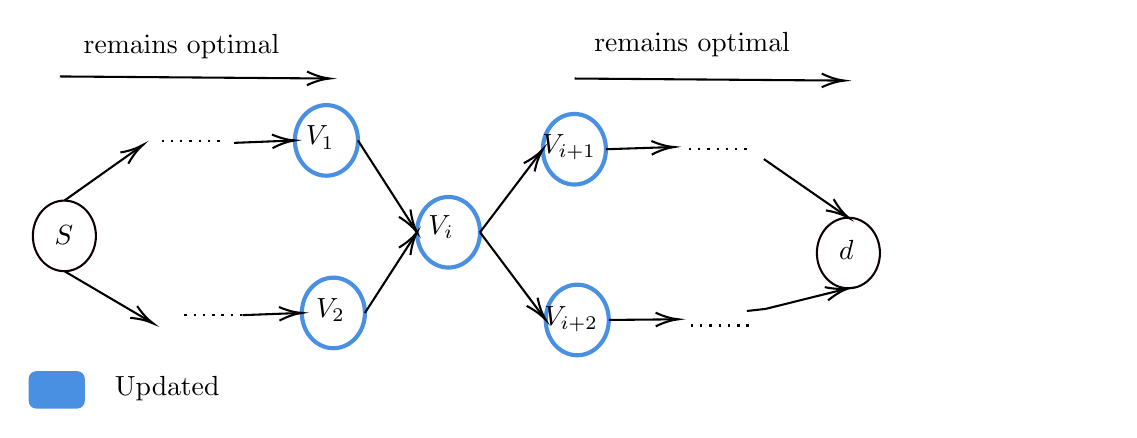
\begin{tikzpicture}[x=0.75pt,y=0.75pt,yscale=-1,xscale=1]
%uncomment if require: \path (0,359); %set diagram left start at 0, and has height of 359

%Shape: Rectangle [id:dp480508071363392] 
\draw  [draw opacity=0][fill={rgb, 255:red, 255; green, 255; blue, 255 }  ,fill opacity=1 ] (572,51) -- (642,51) -- (642,64) -- (572,64) -- cycle ;
%Shape: Rectangle [id:dp03384397152413832] 
\draw  [draw opacity=0][fill={rgb, 255:red, 255; green, 255; blue, 255 }  ,fill opacity=1 ] (573,107) -- (643,107) -- (643,120) -- (573,120) -- cycle ;
%Shape: Ellipse [id:dp9103409908276086] 
\draw  [color={rgb, 255:red, 14; green, 0; blue, 0 }  ,draw opacity=1 ] (125,113.82) .. controls (125,104.43) and (131.8,96.81) .. (140.19,96.81) .. controls (148.57,96.81) and (155.37,104.43) .. (155.37,113.82) .. controls (155.37,123.21) and (148.57,130.82) .. (140.19,130.82) .. controls (131.8,130.82) and (125,123.21) .. (125,113.82) -- cycle ;
%Shape: Ellipse [id:dp740083289005012] 
\draw  [color={rgb, 255:red, 74; green, 144; blue, 226 }  ,draw opacity=1 ][line width=1.5]  (251.25,67.82) .. controls (251.25,58.43) and (258.05,50.81) .. (266.44,50.81) .. controls (274.83,50.81) and (281.63,58.43) .. (281.63,67.82) .. controls (281.63,77.21) and (274.83,84.82) .. (266.44,84.82) .. controls (258.05,84.82) and (251.25,77.21) .. (251.25,67.82) -- cycle ;
%Shape: Ellipse [id:dp9541917593446743] 
\draw  [color={rgb, 255:red, 74; green, 144; blue, 226 }  ,draw opacity=1 ][line width=1.5]  (254.61,150.94) .. controls (254.61,141.55) and (261.41,133.94) .. (269.79,133.94) .. controls (278.18,133.94) and (284.98,141.55) .. (284.98,150.94) .. controls (284.98,160.33) and (278.18,167.94) .. (269.79,167.94) .. controls (261.41,167.94) and (254.61,160.33) .. (254.61,150.94) -- cycle ;
%Shape: Ellipse [id:dp1856273890999922] 
\draw  [color={rgb, 255:red, 74; green, 144; blue, 226 }  ,draw opacity=1 ][line width=1.5]  (310.07,112.07) .. controls (310.07,102.68) and (316.86,95.06) .. (325.25,95.06) .. controls (333.64,95.06) and (340.44,102.68) .. (340.44,112.07) .. controls (340.44,121.46) and (333.64,129.07) .. (325.25,129.07) .. controls (316.86,129.07) and (310.07,121.46) .. (310.07,112.07) -- cycle ;
%Shape: Ellipse [id:dp9526061796743859] 
\draw  [color={rgb, 255:red, 74; green, 144; blue, 226 }  ,draw opacity=1 ][line width=1.5]  (370.73,72.07) .. controls (370.73,62.68) and (377.53,55.06) .. (385.91,55.06) .. controls (394.3,55.06) and (401.1,62.68) .. (401.1,72.07) .. controls (401.1,81.46) and (394.3,89.07) .. (385.91,89.07) .. controls (377.53,89.07) and (370.73,81.46) .. (370.73,72.07) -- cycle ;
%Shape: Ellipse [id:dp044156064147011787] 
\draw  [color={rgb, 255:red, 14; green, 0; blue, 0 }  ,draw opacity=1 ] (502.74,122.07) .. controls (502.74,112.68) and (509.54,105.06) .. (517.93,105.06) .. controls (526.32,105.06) and (533.11,112.68) .. (533.11,122.07) .. controls (533.11,131.46) and (526.32,139.07) .. (517.93,139.07) .. controls (509.54,139.07) and (502.74,131.46) .. (502.74,122.07) -- cycle ;
%Shape: Ellipse [id:dp6843056607618183] 
\draw  [color={rgb, 255:red, 74; green, 144; blue, 226 }  ,draw opacity=1 ][line width=1.5]  (372.1,154.32) .. controls (372.1,144.93) and (378.9,137.32) .. (387.28,137.32) .. controls (395.67,137.32) and (402.47,144.93) .. (402.47,154.32) .. controls (402.47,163.71) and (395.67,171.33) .. (387.28,171.33) .. controls (378.9,171.33) and (372.1,163.71) .. (372.1,154.32) -- cycle ;
%Straight Lines [id:da4109082321511348] 
\draw    (140.19,130.82) -- (181.28,154.99) ;
\draw [shift={(183,156)}, rotate = 210.46] [color={rgb, 255:red, 0; green, 0; blue, 0 }  ][line width=0.75]    (10.93,-3.29) .. controls (6.95,-1.4) and (3.31,-0.3) .. (0,0) .. controls (3.31,0.3) and (6.95,1.4) .. (10.93,3.29)   ;
%Straight Lines [id:da09020512135141656] 
\draw    (140.19,96.81) -- (176.37,71.16) ;
\draw [shift={(178,70)}, rotate = 144.66] [color={rgb, 255:red, 0; green, 0; blue, 0 }  ][line width=0.75]    (10.93,-3.29) .. controls (6.95,-1.4) and (3.31,-0.3) .. (0,0) .. controls (3.31,0.3) and (6.95,1.4) .. (10.93,3.29)   ;
%Straight Lines [id:da07010447777978679] 
\draw    (469,150) -- (478,149) -- (515.99,139.55) ;
\draw [shift={(517.93,139.07)}, rotate = 166.03] [color={rgb, 255:red, 0; green, 0; blue, 0 }  ][line width=0.75]    (10.93,-3.29) .. controls (6.95,-1.4) and (3.31,-0.3) .. (0,0) .. controls (3.31,0.3) and (6.95,1.4) .. (10.93,3.29)   ;
%Straight Lines [id:da3901833128352341] 
\draw    (477.19,76.81) -- (516.28,103.92) ;
\draw [shift={(517.93,105.06)}, rotate = 214.74] [color={rgb, 255:red, 0; green, 0; blue, 0 }  ][line width=0.75]    (10.93,-3.29) .. controls (6.95,-1.4) and (3.31,-0.3) .. (0,0) .. controls (3.31,0.3) and (6.95,1.4) .. (10.93,3.29)   ;
%Straight Lines [id:da5860775319064822] 
\draw    (222,69) -- (249.26,67.9) ;
\draw [shift={(251.25,67.82)}, rotate = 177.68] [color={rgb, 255:red, 0; green, 0; blue, 0 }  ][line width=0.75]    (10.93,-3.29) .. controls (6.95,-1.4) and (3.31,-0.3) .. (0,0) .. controls (3.31,0.3) and (6.95,1.4) .. (10.93,3.29)   ;
%Straight Lines [id:da9472064018730602] 
\draw    (226,152) -- (252.61,151.01) ;
\draw [shift={(254.61,150.94)}, rotate = 177.88] [color={rgb, 255:red, 0; green, 0; blue, 0 }  ][line width=0.75]    (10.93,-3.29) .. controls (6.95,-1.4) and (3.31,-0.3) .. (0,0) .. controls (3.31,0.3) and (6.95,1.4) .. (10.93,3.29)   ;
%Straight Lines [id:da6786123019459969] 
\draw    (281.63,67.82) -- (308.98,110.38) ;
\draw [shift={(310.07,112.07)}, rotate = 237.27] [color={rgb, 255:red, 0; green, 0; blue, 0 }  ][line width=0.75]    (10.93,-3.29) .. controls (6.95,-1.4) and (3.31,-0.3) .. (0,0) .. controls (3.31,0.3) and (6.95,1.4) .. (10.93,3.29)   ;
%Straight Lines [id:da8151696040712353] 
\draw    (284.98,150.94) -- (308.98,113.75) ;
\draw [shift={(310.07,112.07)}, rotate = 122.83] [color={rgb, 255:red, 0; green, 0; blue, 0 }  ][line width=0.75]    (10.93,-3.29) .. controls (6.95,-1.4) and (3.31,-0.3) .. (0,0) .. controls (3.31,0.3) and (6.95,1.4) .. (10.93,3.29)   ;
%Straight Lines [id:da11134508242076424] 
\draw    (340.44,112.07) -- (369.52,73.66) ;
\draw [shift={(370.73,72.07)}, rotate = 127.13] [color={rgb, 255:red, 0; green, 0; blue, 0 }  ][line width=0.75]    (10.93,-3.29) .. controls (6.95,-1.4) and (3.31,-0.3) .. (0,0) .. controls (3.31,0.3) and (6.95,1.4) .. (10.93,3.29)   ;
%Straight Lines [id:da49946303299867534] 
\draw    (340.44,112.07) -- (370.9,152.72) ;
\draw [shift={(372.1,154.32)}, rotate = 233.16] [color={rgb, 255:red, 0; green, 0; blue, 0 }  ][line width=0.75]    (10.93,-3.29) .. controls (6.95,-1.4) and (3.31,-0.3) .. (0,0) .. controls (3.31,0.3) and (6.95,1.4) .. (10.93,3.29)   ;
%Straight Lines [id:da9661195791648898] 
\draw    (401.1,72.07) -- (432,71.06) ;
\draw [shift={(434,71)}, rotate = 178.14] [color={rgb, 255:red, 0; green, 0; blue, 0 }  ][line width=0.75]    (10.93,-3.29) .. controls (6.95,-1.4) and (3.31,-0.3) .. (0,0) .. controls (3.31,0.3) and (6.95,1.4) .. (10.93,3.29)   ;
%Straight Lines [id:da9084929098821986] 
\draw    (402.47,154.32) -- (434,154.02) ;
\draw [shift={(436,154)}, rotate = 179.45] [color={rgb, 255:red, 0; green, 0; blue, 0 }  ][line width=0.75]    (10.93,-3.29) .. controls (6.95,-1.4) and (3.31,-0.3) .. (0,0) .. controls (3.31,0.3) and (6.95,1.4) .. (10.93,3.29)   ;
%Straight Lines [id:da0449100159502247] 
\draw  [dash pattern={on 0.84pt off 2.51pt}]  (187,68) -- (215,68) ;
%Straight Lines [id:da5356080041931417] 
\draw  [dash pattern={on 0.84pt off 2.51pt}]  (198,152) -- (226,152) ;
%Straight Lines [id:da9346868766060579] 
\draw  [dash pattern={on 0.84pt off 2.51pt}]  (441,72) -- (469,72) ;
%Straight Lines [id:da9642012858007416] 
\draw  [dash pattern={on 0.84pt off 2.51pt}]  (442,157) -- (470,157) ;
%Rounded Rect [id:dp6788726220855428] 
\draw  [draw opacity=0][fill={rgb, 255:red, 74; green, 144; blue, 226 }  ,fill opacity=1 ] (123,182.6) .. controls (123,180.61) and (124.61,179) .. (126.6,179) -- (146.4,179) .. controls (148.39,179) and (150,180.61) .. (150,182.6) -- (150,193.4) .. controls (150,195.39) and (148.39,197) .. (146.4,197) -- (126.6,197) .. controls (124.61,197) and (123,195.39) .. (123,193.4) -- cycle ;
%Straight Lines [id:da6555072227430381] 
\draw    (138,37) -- (266,37.98) ;
\draw [shift={(268,38)}, rotate = 180.44] [color={rgb, 255:red, 0; green, 0; blue, 0 }  ][line width=0.75]    (10.93,-3.29) .. controls (6.95,-1.4) and (3.31,-0.3) .. (0,0) .. controls (3.31,0.3) and (6.95,1.4) .. (10.93,3.29)   ;
%Straight Lines [id:da6809797244968319] 
\draw    (386,38) -- (514,38.98) ;
\draw [shift={(516,39)}, rotate = 180.44] [color={rgb, 255:red, 0; green, 0; blue, 0 }  ][line width=0.75]    (10.93,-3.29) .. controls (6.95,-1.4) and (3.31,-0.3) .. (0,0) .. controls (3.31,0.3) and (6.95,1.4) .. (10.93,3.29)   ;

% Text Node
\draw (134,107.4) node [anchor=north west][inner sep=0.75pt]    {$S$};
% Text Node
\draw (255,59.4) node [anchor=north west][inner sep=0.75pt]    {$V_{1}$};
% Text Node
\draw (260,142.4) node [anchor=north west][inner sep=0.75pt]    {$V_{2}$};
% Text Node
\draw (314,102.4) node [anchor=north west][inner sep=0.75pt]    {$V_{i}$};
% Text Node
\draw (369,63.4) node [anchor=north west][inner sep=0.75pt]    {$V_{i+1}$};
% Text Node
\draw (370,146.4) node [anchor=north west][inner sep=0.75pt]    {$V_{i+2}$};
% Text Node
\draw (512,114.4) node [anchor=north west][inner sep=0.75pt]    {$d$};
% Text Node
\draw (163,180) node [anchor=north west][inner sep=0.75pt]   [align=left] {Updated};
% Text Node
\draw (148,15) node [anchor=north west][inner sep=0.75pt]   [align=left] {remains optimal};
% Text Node
\draw (394,14) node [anchor=north west][inner sep=0.75pt]   [align=left] {remains optimal};


\end{tikzpicture}